\documentclass{article}

\usepackage{tikz}
\usetikzlibrary{arrows}

\begin{document}



\begin{figure}
\centering
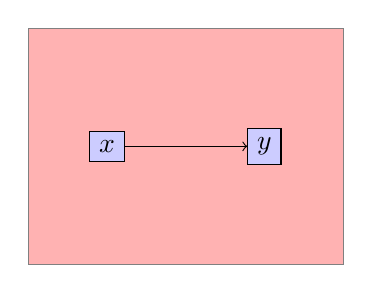
\begin{tikzpicture}[node distance=2.5cm]
\filldraw[fill=red!30,draw=gray] (-2,-1.5) rectangle(2,1.5);
    \node [draw, fill=blue!20] (a) at (-1,0) {$x$};
    \node [draw, fill=blue!20] (b) at (+1,0) {$y$};
    \draw[->] (a)--(b);
\end{tikzpicture}
\caption{A tikz example}
\end{figure}

\end{document}